\documentclass[pdf, handout]{beamer}
\mode<presentation>{\usetheme{Warsaw}}
%% preamble
 \setbeamertemplate{headline}{}
\setbeamertemplate{section page}[mine]

\setbeamertemplate{footline}[frame number]
\title{Valuation of Options - part 2}
\subtitle{Quantitative Finance}
\author{Tilburg University}
\institute{Ramon van den Akker}
\date{}
%%
\usepackage{array}
\usepackage{multirow}
\usepackage{amsmath}
\usepackage{multicol}
\usepackage{subfigure}
\usepackage{graphicx}
\usepackage{pstricks}
\input{commands.txt}
\newcommand{\Var}{\operatorname{Var}}
\renewcommand{\epsi}{\varepsilon}
\newcommand{\argmin}{\mathop{\mathrm{arg\,min}}}
\newcommand{\rank}{\operatorname{rank}}
\renewcommand{\kansp}{\mathbb{P}}
\renewcommand{\calF}{\mathcal{F}}
\newcommand{\e}{\operatorname{e}}
\newcommand{\Bin}{\operatorname{Bin}}
\newcommand{\kbin}{\operatorname{b}}
\newcommand{\lin}{\operatorname{lin}}
\newcommand{\kansq}{\mathbb{Q}}
\DeclareMathOperator*\ster{*} \DeclareMathOperator*\argmax{argmax}
\usepackage{color}
\AtBeginSection{\frame{\sectionpage}}
\newtranslation[to=greek]{Section}{En'othta}
\newtranslation[to=greek]{Subsection}{Upoen'othta}
\defbeamertemplate{section page}{mine}[1][]{%
  \begin{centering}
    {\usebeamerfont{section name}\usebeamercolor[fg]{section name}#1}
    \vskip1em\par
    \begin{beamercolorbox}[sep=12pt,center]{part title}
      \usebeamerfont{section title}\insertsection\par
    \end{beamercolorbox}
  \end{centering}
}
\defbeamertemplate{subsection page}{mine}[1][]{%
  \begin{centering}
    {\usebeamerfont{subsection name}\usebeamercolor[fg]{subsection name}#1}
    \vskip1em\par
    \begin{beamercolorbox}[sep=8pt,center,#1]{part title}
      \usebeamerfont{subsection title}\insertsubsection\par
    \end{beamercolorbox}
  \end{centering}
}

\begin{document}

\begin{frame}
\titlepage
\end{frame}

\begin{frame}{Assumptions  Black-Scholes market (recap)}
In class we will almost exclusively work with the `Black-Scholes market'.
\\ \vspace{.5cm}
\textbf{Assumptions on price processes:} \\
Asset price:
\[
\rd S_t=\mu S_t \rd t + \sigma S_t \rd W_t,\quad S_0=s_0,\,\,\, \var(W_1) = 1
\]
Money Market Account:
\[
\rd B_t= r B_t \rd t,\quad B_0=1
\]
\textbf{Assumptions on market:} \\
\begin{itemize}
\item frictionless trading
\begin{itemize}
\item no transaction costs
\item trading in continuous-time possible
\item no restrictions on short sales and fractional positions
\end{itemize}
\item borrowing rate = lending rate
\end{itemize}
\end{frame}
%
%\begin{frame}[toc=multivariate]{Multivariate case}
%$k$ risky assets with dynamics
%\[
%\rd S_{i,t}=\mu_i S_{i,t} \rd t + \sigma_i S_{i,t} \rd W_{i,t},
%\]
%where $W=(W_1,\dots,W_k)$ is a standard multivariate Brownian
%motion with $\cov (W_{i,t}, W_{j,t})=\rho_{ij}\sigma_i\sigma_j
%t$
%\end{frame}

\begin{frame}{Agenda}
\begin{itemize}
\item we are interested in  price $C_t$ of (European) option with payoff $C_T=h(S_T)$
\item we will discuss three methods to determine fair price (using continuous-time model for financial market):
\begin{itemize}
\item Black-Scholes Partial Differential Equation
\item risk-neutral pricing
\item pricing kernel
\end{itemize}
\textbf{These slides discuss the Black-Scholes Partial Differential Equation approach.}
\end{itemize}
\end{frame}

\section[toc=Black-Scholes PDE]{The Black-Scholes Partial Differential Equation}

\begin{frame}{The problem}
\textbf{Setup:}
\begin{itemize}
\item Black-Scholes market (1 risky asset)
\item we restrict to
Markovian trading strategies:
\[
\phi_t=\tilde\phi(B_t, S_t)= \phi(t,S_t) \text{ and } \psi_t=\tilde\psi(B_t, S_t)
=\psi (t, S_t)
\]
So we can write, for some function $F$,
\[
 V_t=\phi(t, S_t) S_t + \psi_t(t, S_t) B_t=F(t, S_t)
\]
\end{itemize}
\textbf{Question:} \\
Which $F$'s correspond to \textbf{self-financing} trading strategies?
\\ \vspace{.25cm}
\textbf{Why interesting?}
\begin{itemize}
\item consider option with payoff $h(S_T)$ at maturity
\item if we can find self-financing portfolio with $F(T, S_T)= h(S_T)$ then
no-arbitrage price of option at time $0\leq t <T$ is given by
\[
C_t=F(t, S_t)
\]
\end{itemize}
\end{frame}

\begin{frame}{Black-Scholes Partial Differential Equation}
\textbf{Black-Scholes Partial Differential Equation:} \\
$F$ corresponds to a self-financing trading strategy if and only if $F$ is a solution to the Partial Differential Equation (equation with function $G$ as variable)
\[
\frac{\partial G}{\delta t}(t, s) + r s \frac{\partial G}{\partial
s}(t, s) + \frac{1}{2}\sigma^2 s^2 \frac{\partial^2 G}{\partial
s^2}(t,s) -r G(t,s )=0\,\, \forall s>0, t\in[0, T),
\]
and in that case the positions in the self-financing trading strategy are given by:
\[
\phi(t,s)=\frac{\partial F}{\partial s}(t, s),
\]
and
\[
\psi(t,s)=\frac{F(t,s)-\phi(t,s) s}{\exp(rt)}.
\]
\\ \vspace{.3cm}
\textbf{Remarks:}
\begin{itemize}
\item  $\mu$ does not play a role!
\item using different models (i.e. SDEs)
for $B$ and $S$ leads, in general, to
different PDE!
\end{itemize}
\end{frame}

\begin{frame}{Derivation of the PDE}
Which $F$ are possible (when using self-financing strategies $(\phi(t,S_t),\psi(t,S_t))$)?
We have
\begin{itemize}
\item[(1)] $V_t=F(t,S_t)$
\item[(2)] $\rd V_t= \phi(t,S_t) \rd S_t + \psi(t,S_t) \rd B_t$
\end{itemize}
\vspace{-.2cm}
\begin{itemize}
\item apply It\^{o} to (1) and insert $\rd S_t$  $\implies$
$
\rd V_t=\textcolor{blue}{a_t} \rd t + \textcolor{red}{b_t} \rd W_t
$
\item insert $\rd S_t$ and $\rd B_t$ in RHS of (2) $\implies$
$\rd V_t=\textcolor{blue}{c_t} \rd t + \textcolor{red}{d_t} \rd W_t$
\item obtain system of equations
\[
\left\{
  \begin{array}{ll}
    a_t=c_t  \\
    b_t=d_t % \\
%    (1).
  \end{array}
\right.
\]
\item solving $\implies$ conditions on $F$ (PDE)
\end{itemize}
\end{frame}

\begin{frame}{Warning: sloppy notation}
We will often use the following notations/abbrevations when working with PDEs:
\begin{itemize}
\item $F_S = (\partial F / \partial s) = (\partial F / \partial s)(t,S_t)$
\item $F_t = (\partial F / \partial t) = (\partial F / \partial t)(t,S_t)$
\item $F = F(t,S_t$)
\item etc.
\end{itemize}
The notation $F_t$ is somewhat confusing as it seems to refer to a stochastic process. And you argue that it would be a natural abbrevation for $F(t,S_t)$. \\
If you want to be clear and safe it could be better to just write down the partial derivatives fully.
\end{frame}


\begin{frame}{Derivation}
%{\small
We have
\begin{itemize}
\item[(1)] $V_t=F(t,S_t)$
\item[(2)] $\rd V_t= \phi(t,S_t) \rd S_t + \psi(t,S_t) \rd B_t$
\end{itemize}
\vspace{-.2cm}
\begin{itemize}
\item apply It\^{o} to (1) and insert $\rd S_t = \mu S_t \rd t + \sigma S_t \rd W_t$  $\implies$
\begin{align*}
\rd V_t &= F_S \rd S_t + F_t \rd t + \frac{1}{2} F_{SS} \rd [S,S]_t 
\\
&=  \left( F_S \mu S_t +F_t +  \frac{1}{2} F_{SS} \sigma^2 S_t^2  \right) 
\rd t + F_S \sigma S_t \rd W_t 
\end{align*}
\item insert $\rd S_t$ and $\rd B_t=rB_t\rd t$ in RHS of (2) $\implies$
\begin{align*}
\rd V_t &= (\phi_t \mu S_t + r\psi_t B_t) \rd t +  \phi_t \sigma S_t \rd W_t
\end{align*}
\item hence $\phi_t = \phi(t,S_t) = F_{S}(t,S_t)=F_S$
\item and
\begin{align*}
F_S \mu S_t +F_t +  \frac{1}{2}\sigma^2 F_{SS} S_t^2    
&= \phi_t \mu S_t + r\psi_t B_t
\end{align*}
\end{itemize}
%}
\end{frame}



\begin{frame}{Derivation}
We need to prove
\[
\frac{\delta F}{\delta t}(t,s) + r s \frac{\partial F}{\partial
s}(t,s) + \frac{1}{2}\sigma^2 s^2 \frac{\partial^2 F}{\partial
s^2}(t,s) -r F(t,s)=0\quad \forall s>0,\,t\in[0, T),
\]
On the previous slide we obtained
\begin{align*}
F_t + \frac{1}{2}\sigma^2 F_{SS} S_t^2    
&=  r\psi_t B_t.
\end{align*}
As $\psi_t B_t = F - \phi_t S_t = F - F_S S_t$
we obtain the result.
\end{frame}



\begin{frame}{Alternative Derivation}
\begin{itemize}
\item sell (write) and hold 1 option with price process
$C_t = F(t, S_t)$  (assumption!)
\item let $\phi_t$ be number of stocks at time $t$ and $\psi_t$ the position in the MMA 
\item yields portfolio value $V_t =  - C_t + \phi_t S_t + \psi_t B_t$
\item this portfolio is self-financing if
\[
\rd V_t =  - \rd C_t  + \phi_t \rd S_t + \psi_t \rd B_t
\]
\item 
using It\^o:
\[
\rd V_t = - F_S \rd S_t - F_t \rd t - \frac{1}{2}F_{SS} \rd [S,S]_t + \phi_t \rd S_t
+ \psi_t r B_t \rd t
\]
\item can only eliminate local risk ($\rd W_t$) for $\phi_t = F_S(t, S_t)$!
\item yields $\rd V_t = \cdots \rd t$  which has (locally) no risk, so
rate of return is same as on $B$ $\implies$ $\rd V_t =r V_t \rd t$
\item hence 
\[
-F_t - \frac{1}{2}F_{SS}\sigma^2 S_t^2 + r\psi_t B_t = r \left(  - F  + F_S S_t + \psi_t B_t
\right)
\]
which yields Black-Scholes PDE
\end{itemize}

\end{frame}


\begin{frame}{Application}
Given is a European option with payoff $h(S_T)$ at expiration date/maturity $T$. How can we use the PDE to obtain the price of this option? 
\begin{itemize}
\item Solve the  PDE,
\[
\frac{\delta G}{\delta t}(t, s) + r s \frac{\partial G}{\partial
s}(t, s) + \frac{1}{2}\sigma^2 s^2 \frac{\partial^2 G}{\partial
s^2}(t,s) -r G(t,s )=0,
\]
for all $s>0$, $t\in[0,T)$,
under the boundary condition
\[
G(T,s)=h(s) \text{ for all } s>0.
\]
\item If $F$ is solution to PDE satisfying the boundary condition, then no-arbitrage implies that the price of the option at time $t\in [0, T)$ is given by $F(t, S_t)$.
\item If you are lucky: 'closed-form' solution can be found
\begin{itemize}
\item there is relation to well studied  heat equation
\end{itemize}
\item unlucky:
use numerical techniques; see notebook
\end{itemize}
\end{frame}
%
\begin{frame}{Examples: closed-form solutions}
\begin{itemize}
\item $h(S_T)=S_T$
\[
F(t,s)=s
\]
\item European call option: $h(S_T)=\max\{ S_T-K,0\}$
\[
F(t,s)=s\Phi(d_1)-\exp(-r(T-t))K\Phi(d_2),
\]
with
$d_1=d_2+\sigma\sqrt{T-t}$ and
\[
d_2=\frac{
\log(s/K)+(r-0.5 \sigma^2)(T-t)}{\sigma\sqrt{T-t}}
\]
%\begin{itemize}
%\item see solution to LN Exercise 11.8.1iii (provided on Blackboard)
%\end{itemize}
\end{itemize}
\end{frame}
%
\begin{frame}{Examples: European digital call option}
\begin{itemize}
\item payoff: $h(S_T)=1\{S_T\geq K\}$
\item the B-S PDE can be solved explictly:
\[
F(t,s)=\exp(-r(T-t))\Phi(d_2),
\]
with
\[
d=\frac{
\log(s/K)+(r-0.5 \sigma^2)(T-t)}{\sigma\sqrt{T-t}}
\]
\item
Probability that option ends in-the-money:
\[
\mathbb{P}\{S_T\geq K\}=\Phi\left(
\frac{
\log(s/K)+(\mu-0.5 \sigma^2)(T-t)}{\sigma\sqrt{T-t}}\right)
\]
\end{itemize}
\textbf{In the exercise set you will be asked to verify that $F$ is a solution to the B-S PDE.}
\end{frame}

\begin{frame}{Examples: European digital put option}
Price of the option (at $t=0$) $F(0,s)$ - numerical solution compared to exact solution:
\begin{figure}
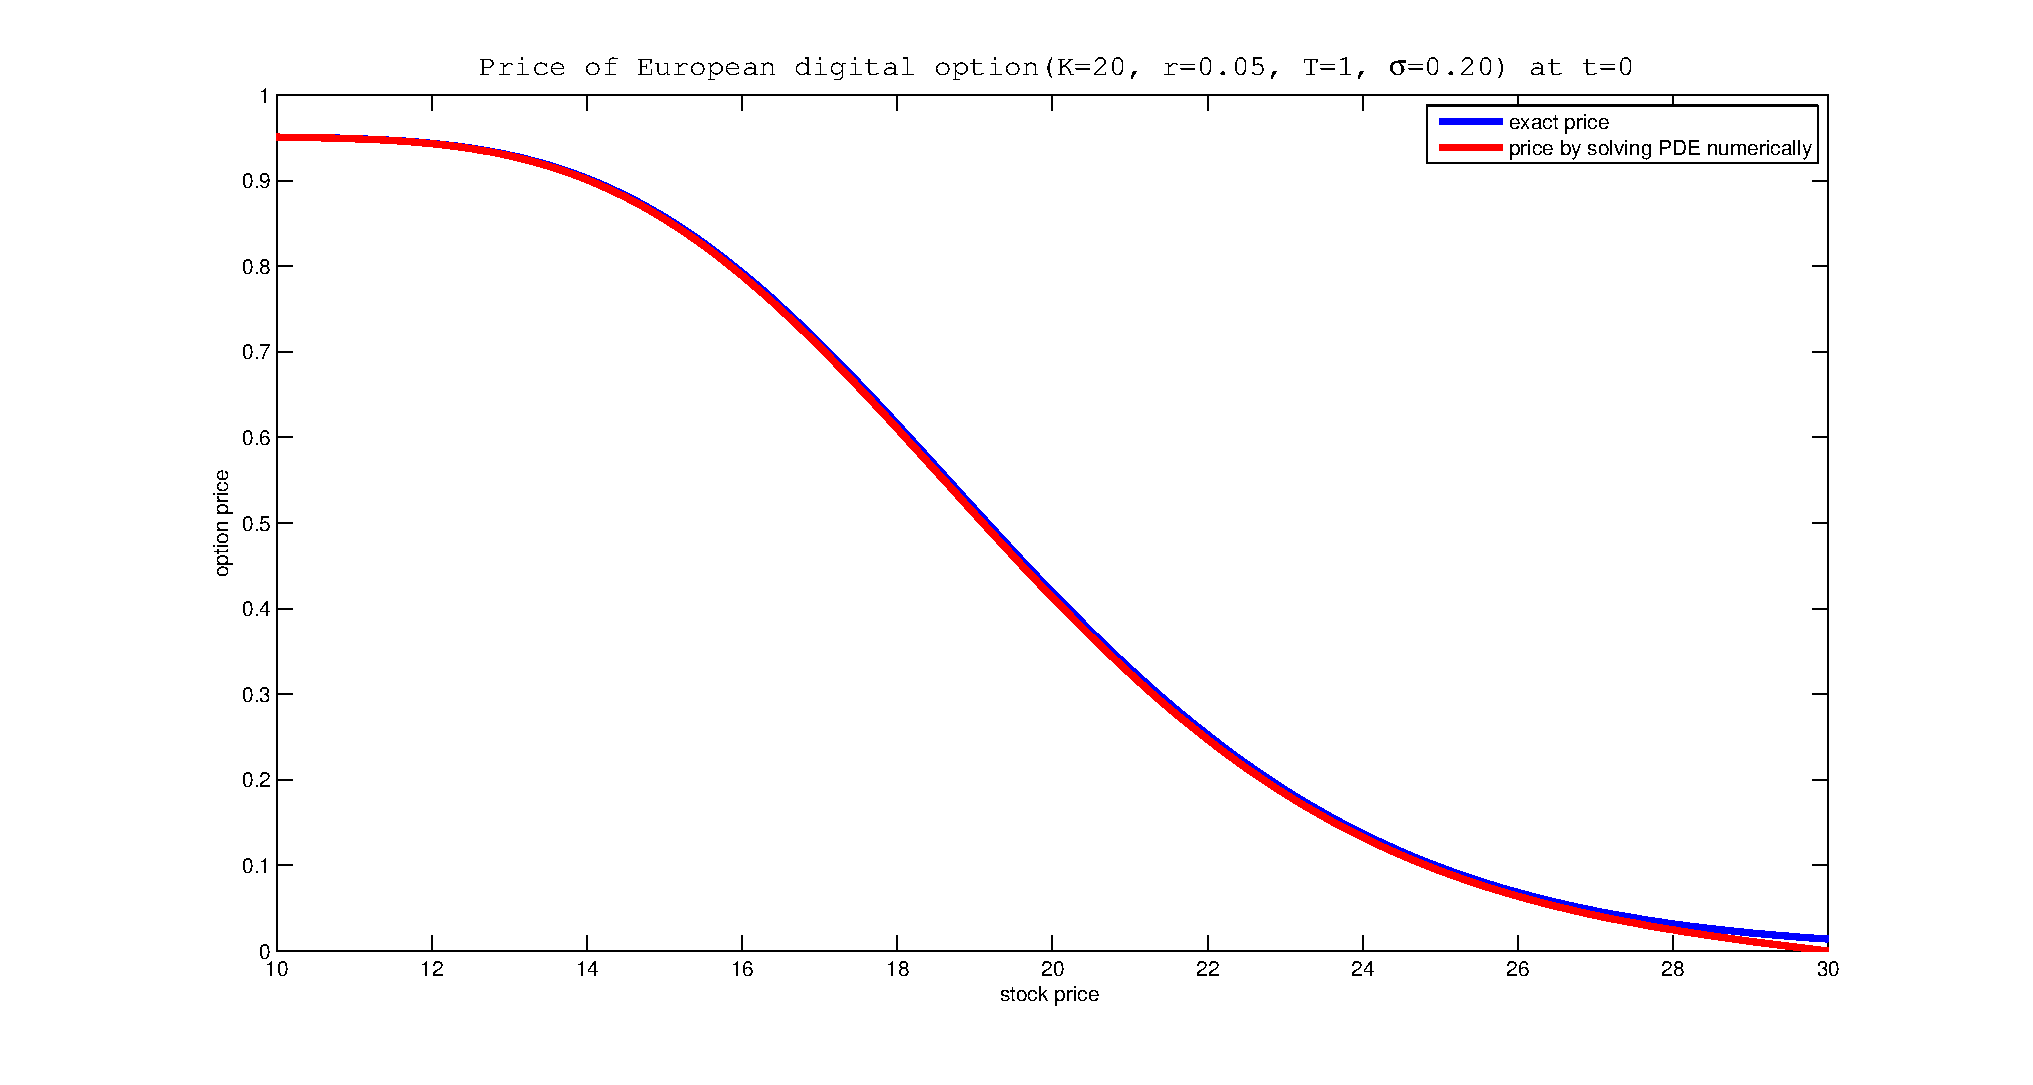
\includegraphics[width=0.85\textwidth]{startprice_dig_put.eps}
\end{figure}
The Group Assignment might contain an exercise on solving the PDE numerically.
\end{frame}

\begin{frame}{Examples: European digital put option}
Value function $F(t,s)$:
\begin{figure}
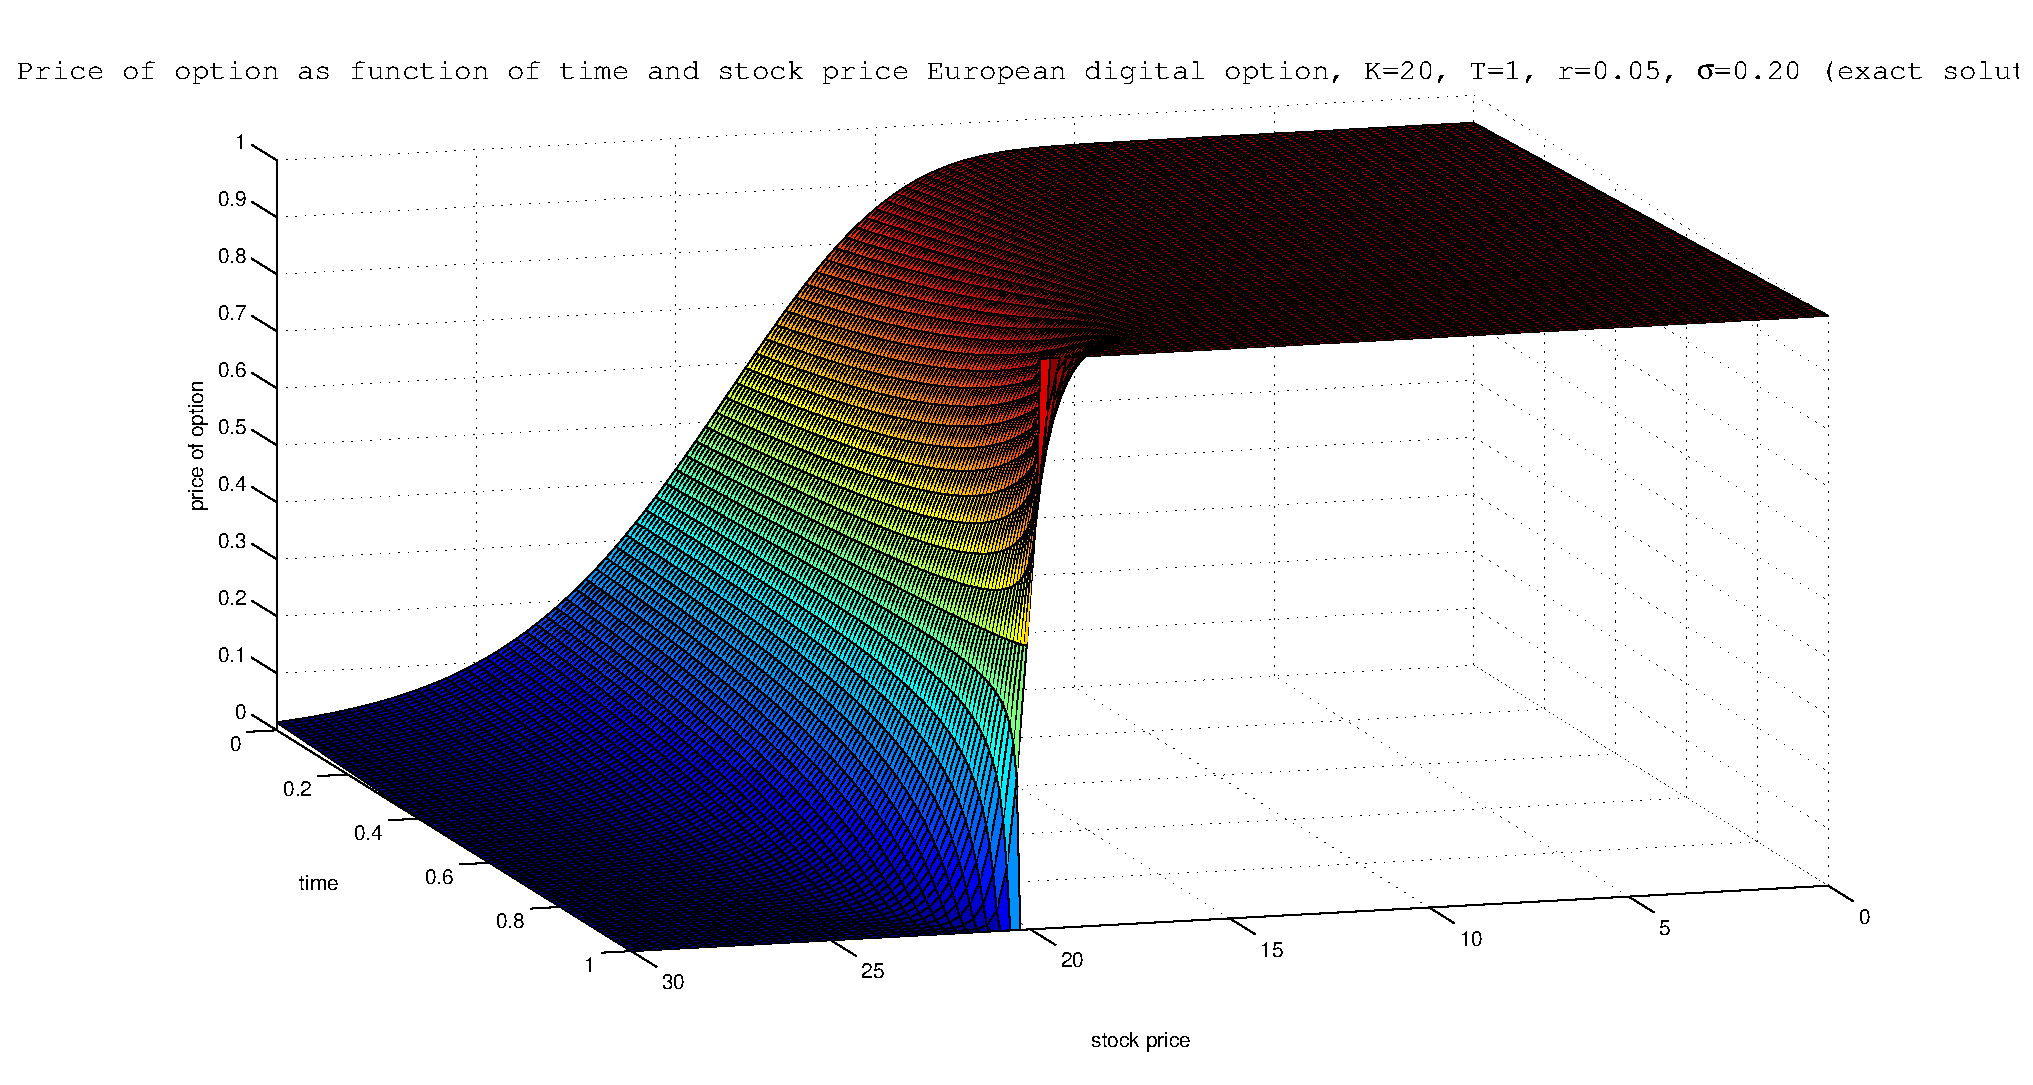
\includegraphics[width=0.85\textwidth]{value_dig_put.eps}
\end{figure}
\end{frame}

\begin{frame}{Feynman-Kac Theorem}
Let $\alpha(t, x)$, $\beta(t,x)$, and $k(t,x)$ be  functions satisfying `regularity conditions'.
Consider the PDE
\[
\frac{\partial G}{\delta t}(t, x) +  \alpha(t, x) \frac{\partial G}{\partial
x}(t, x) + \frac{1}{2} \beta^2(t,x)  \frac{\partial^2 G}{\partial
x^2}(t,x) - k(t, x)  G(t,x )=0, 
\]
for all $x$ and 
$t\in[0, T)$ with boundary condition $G(T, x) = h(x)$ for all $x$.  

Then the solution is given by:
\[
G(t,x)= \mathbb{E}\left[ 
 \exp\left( -  \int_t^T k(s, X_s) \rd s  \right) h( X_T)
\mid X_t=x
\right],
\]
where $X$ is a stochastic process, on the time interval $[t, T]$, defined via the SDE
\[
\rd X_u = \alpha(u,X_u) \rd u + \beta(u, X_u) \rd W_u
\]
and with starting value $X_t=x$, and
where $W$ is a standard Brownian motion.
\end{frame}



\begin{frame}{Black-Scholes PDE reconsidered}
The no-arbitrage price, at time $t\in [0,T)$, of a European option with payoff $h(S_T)$ at expiration date $T>0$ is given by
$F(t, S_t)$ where $F$ satisfies
\[
\frac{\delta F}{\delta t}(t,s) + r s \frac{\partial F}{\partial
s}(t,s) + \frac{1}{2}\sigma^2 s^2 \frac{\partial^2 F}{\partial
s^2}(t,s) -r F(t,s)=0\quad \forall s>0,\,t\in[0, T),
\]
Feynman-Kac tells us that we have
\[
F(t, s)= \mathbb{E}\left[ \e^{-r(T-t)}
 h( S_T)
\mid S_t=s
\right],
\]
where $S$ is defined via the SDE
\[
\rd S_u = r S_u \rd u + \sigma S_u \rd W_u, \quad S_t=s,
\]
where $W$ is a standard Brownian motion.
\end{frame}

\end{document}
